 \documentclass[aspectratio=169]{beamer}

% Must be loaded first
\usepackage{tikz}
\usetikzlibrary{shapes,arrows,positioning,fit,calc}

\usepackage[utf8]{inputenc}
\usepackage{textpos}

% Font configuration
\usepackage{fontspec}

\usepackage[listings, minted]{tcolorbox}
\usepackage{smartdiagram}
\usepackage[export]{adjustbox}

\input{font.tex}

% Tikz for beautiful drawings
\usetikzlibrary{mindmap,backgrounds}
\usetikzlibrary{arrows.meta,arrows}
\usetikzlibrary{shapes.geometric}

% Minted configuration for source code highlighting
\usepackage{minted}
\setminted{highlightcolor=orange!50, linenos}
\setminted{style=lovelace}

\usepackage[listings, minted]{tcolorbox}
\tcbset{left=6mm}

% Use the include theme
\usetheme{codecentric}

% Metadata
\title{Textanalysis with Monoids}
\author{Markus Hauck (@markus1189)}

% The presentation content
\begin{document}

\begin{frame}[noframenumbering,plain]
  \titlepage{}
\end{frame}

\section{Introduction}\label{sec:introduction}

\begin{frame}
  \begin{center}
    {\Huge Textanalysis with Monoids\\}
    (A taste of FP)
  \end{center}
\end{frame}

\begin{frame}
  \frametitle{Introduction}
  \begin{itemize}
  \item IT Consultant at codecentric since >3 years
  \item working in \textbf{Scala} since >5 years, \textbf{Haskell} for fun
  \item passionate functional programmer
  \item Scala and Haskell Meetup in Frankfurt \textemdash{} Say Hi!
  \end{itemize}
\end{frame}

\section{Prelude}\label{sec:prelude}

\begin{frame}
  \begin{center}
    
\includegraphics[width=0.35\textwidth]{static-images/want-you.jpg}
  \end{center}
\end{frame}

\begin{frame}
  \frametitle{Content}
  \begin{itemize}
  \item next slides: why FP?\@
  \item typeclasses (?)
  \item monoids
  \item case study: text analysis
  \item extensions
  \item conclusion
  \end{itemize}
\end{frame}

\begin{frame}[t]
  \frametitle{Lego vs Duplo}
  \begin{center}
    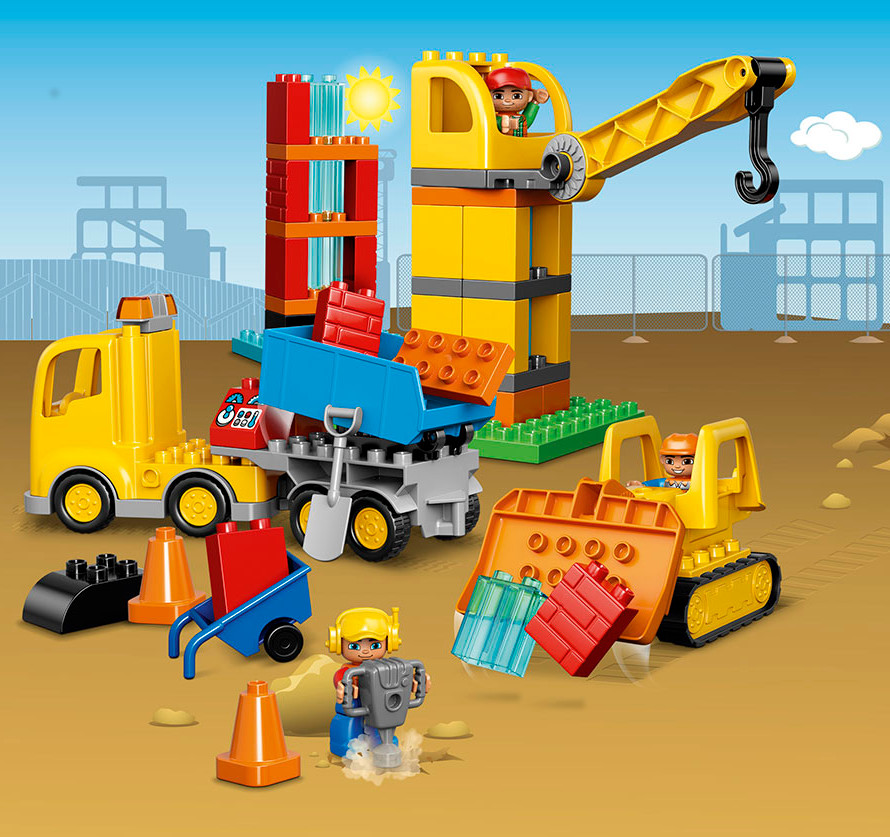
\includegraphics[width=0.48\textwidth]{static-images/duplo-construction.jpg}
    \hspace{1mm}
    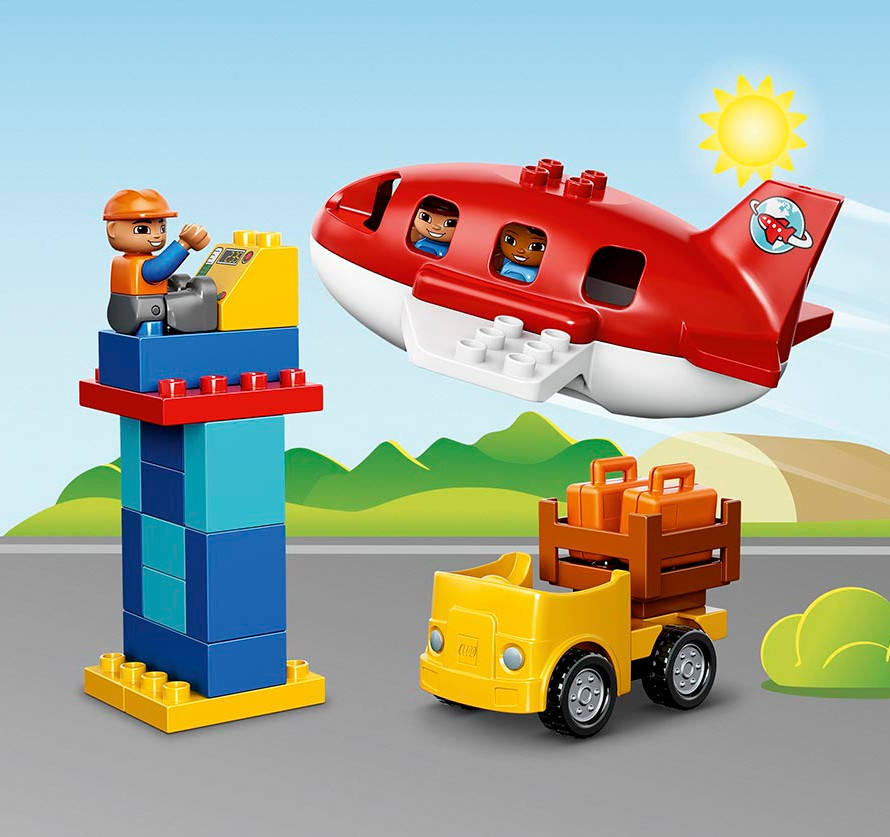
\includegraphics[width=0.48\textwidth]{static-images/duplo-airport.jpg}
  \end{center}
  \vspace{3mm}
  \begin{center}
    {\tiny pictures from \url{shop.lego.com}}
  \end{center}
\end{frame}

\begin{frame}[t]
  \frametitle{Lego vs Duplo}
  \begin{center}
    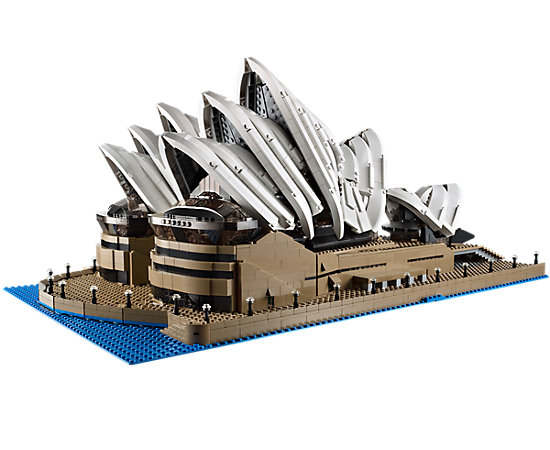
\includegraphics[width=0.49\textwidth]{static-images/lego-sydney-opera.jpg}
    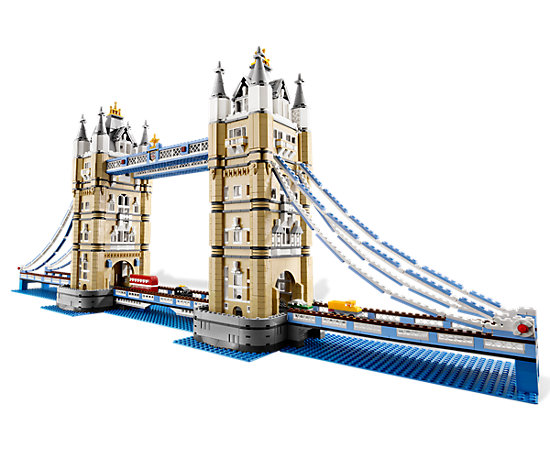
\includegraphics[width=0.49\textwidth]{static-images/lego-tower-bridge.jpg}
  \end{center}
  \vspace{3mm}
  \begin{center}
    {\tiny pictures from \url{shop.lego.com}}
  \end{center}
\end{frame}

\begin{frame}
  \frametitle{Lego vs Duplo}
  \begin{itemize}
  \item<1-> \textbf{Duplo} favours large specialized building blocks
    \begin{itemize}
    \item<1-> blocks tend to be too big
    \item<1-> limited reuse
    \end{itemize}
  \item<2-> \textbf{Lego} focuses on small composable building blocks
    \begin{itemize}
    \item<2-> blocks can conveniently be reused for other purposes
    \item<2-> limited use of specialized building blocks
    \end{itemize}
  \end{itemize}
  \onslide<3->
  \vfill
  \begin{center}
    \textbf{OO} tends to be like \textbf{Duplo}, \textbf{FP} tends to
    be like \textbf{Lego}
  \end{center}
\end{frame}

\begin{frame}
  \frametitle{Typeclasses}
  \begin{itemize}
  \item forget the ``class'' part again (too overloaded)
  \item a way to implement overloaded functions
  \item not (yet) first class in scala
  \item encoded as class/trait with abstract methods
  \item use implicit resolution to define and pass around instances
  \end{itemize}
\end{frame}

\begin{frame}[fragile]
  \frametitle{Typeclasses}
  \begin{minted}{scala}
abstract class Showable[A] {
  def show(x: A): String
}

object Showable {
  implicit val showableInt = new Showable[Int] {
    def show(x: Int): String = x.toString
  }
}
  \end{minted}
\end{frame}

\begin{frame}
  \frametitle{Typeclasses}
  \begin{itemize}
  \item disclaimer: if you want to nitpick, ``Int is a <TC-Name>'' is wrong
  \item {State,Option,List} is \textbf{not} a Monad
  \item correct: {State,Option,List} has a (valid) Monad instance
  \item is that all? No \textemdash{} laws
  \end{itemize}
\end{frame}

\begin{frame}
  \frametitle{Typeclasses \textemdash{} Laws}
  \begin{itemize}
  \item typeclasses need laws
  \item otherwise it is super hard to reason about code
  \item at least without knowing all the instances (impossible)
  \item that's why custom typeclasses without laws are frowned upon
  \item there are still reasons, but mostly: \textbf{don't unless you know why}
  \end{itemize}
\end{frame}

\section{Case Study}

\begin{frame}[fragile]
  \frametitle{The Case Study}
  \begin{itemize}
  \item analyze text file/stream/\ldots{}
  \item collect multiple metrics
  \item using single traversal
  \item similar to the \texttt{wc} commandline tool
  \end{itemize}
  \begin{minted}{sh}
bash> wc moby-dick.txt
21206  208425 1193382 moby-dick.txt
  \end{minted}
\end{frame}

\begin{frame}[fragile]
  \frametitle{Monoids}
  \begin{center}
    \begin{minted}{scala}
     0  +       1  +       5
     1  *       2  *       5
    ""  + "Hello"  + "World"
List() ++ List(4) ++ List(2)
    \end{minted}
  \end{center}
\end{frame}

\begin{frame}
  \frametitle{Monoids}
  \begin{itemize}
  \item claim: most of you are using them without knowing it
  \item \textbf{very} common pattern
  \item implemented as a typeclass + instances
  \item provided by FP libraries (cats)
  \end{itemize}
\end{frame}

\begin{frame}[fragile]
  \frametitle{Monoids}
  \begin{itemize}
  \item Quick Recap: Monoids
  \item binary method \texttt{combine} and nullary method \texttt{empty}
    \vspace{1cm}
    \begin{minted}{scala}
trait Monoid[A] {
  def empty: A
  def combine(x: A, y: A): A
}

// infix operator: x |+| y === combine(x, y)
    \end{minted}
  \end{itemize}
\end{frame}

\begin{frame}[fragile]
  we need to implement:
  \begin{minted}{scala}
implicit val intMonoid: Monoid[Int] = new Monoid[Int] {
  def empty: Int = ???
  def combine(x: Int, y: Int): Int = ???
}
  \end{minted}
\end{frame}

\begin{frame}[fragile, noframenumbering]
  \begin{itemize}
  \item  what about
  \end{itemize}
  \begin{minted}{scala}
implicit val intMonoid: Monoid[Int] = new Monoid[Int] {
  def empty: Int = 42
  def combine(x: Int, y: Int): Int = 1337
}
\end{minted}
\begin{itemize}
\item that's what laws are for
\item check using ScalaCheck / Discipline / \ldots{}
\end{itemize}
\end{frame}

\begin{frame}[fragile]
  \frametitle{Monoid Laws}
  \begin{minted}{scala}
empty |+|     y === y                (left identity)
x     |+| empty === x                (right identity)
(x |+| y) |+| z === x |+| (y |+| z)  (associative)
  \end{minted}
  \begin{itemize}
  \item associativity: it's about order of \textbf{evaluation}
  \item not: commutativity, where order of operands does not matter
  \end{itemize}
\end{frame}

\begin{frame}[fragile, noframenumbering]
  \begin{minted}{scala}
implicit val intMonoid: Monoid[Int] = new Monoid[Int] {
  def empty: Int = 0
  def combine(x: Int, y: Int): Int = ???
}
  \end{minted}
\end{frame}

\begin{frame}[fragile, noframenumbering]
  \begin{minted}{scala}
implicit val intMonoid: Monoid[Int] = new Monoid[Int] {
  def empty: Int = 0
  def combine(x: Int, y: Int): Int = x + y
}
  \end{minted}
\end{frame}

\begin{frame}[fragile, noframenumbering]
  \begin{minted}{scala}
implicit val intMonoid: Monoid[Int] = new Monoid[Int] {
  def empty: Int = 1
  def combine(x: Int, y: Int): Int = ???
}
  \end{minted}
\end{frame}

\begin{frame}[fragile, noframenumbering]
  \begin{minted}{scala}
implicit val intMonoid: Monoid[Int] = new Monoid[Int] {
  def empty: Int = 1
  def combine(x: Int, y: Int): Int = x * y
}
  \end{minted}
\end{frame}

\begin{frame}[fragile, noframenumbering]
  \begin{minted}{scala}
implicit val intMonoid: Monoid[Int] = new Monoid[Int] {
  def empty: Int = Int.MinValue
  def combine(x: Int, y: Int): Int = ???
}
  \end{minted}
\end{frame}

\begin{frame}[fragile, noframenumbering]
  \begin{minted}{scala}
implicit val intMonoid: Monoid[Int] = new Monoid[Int] {
  def empty: Int = Int.MinValue
  def combine(x: Int, y: Int): Int = x.max(y)
}
  \end{minted}
\end{frame}

\begin{frame}[fragile]
  \begin{center}
    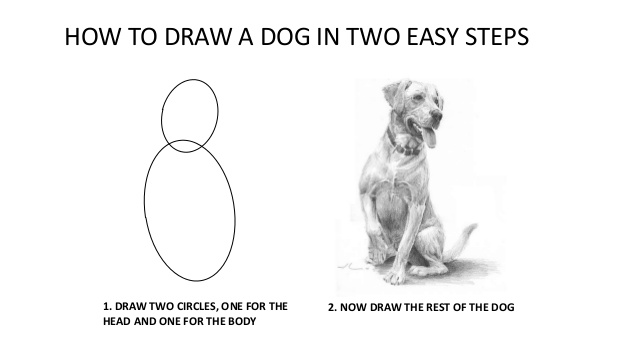
\includegraphics[width=0.8\textwidth]{static-images/draw-dog.jpg}
  \end{center}
\end{frame}

\begin{frame}[fragile]
  \frametitle{Monoids}
  \begin{center}
    \begin{minted}{scala}
Monoid.empty |+|       1 |+|       5
Monoid.empty |+|       2 |+|       5
Monoid.empty |+| "Hello" |+| "World"
Monoid.empty |+| List(4) |+| List(2)
    \end{minted}
  \end{center}
\end{frame}

\begin{frame}[fragile,t]
  \frametitle{Monoids: Counting Chars}
  \begin{itemize}
  \item counting chars is easy, use \texttt{(Int, +)} as a Monoid
  \item count 1 (\texttt{combine} 1) for every character
  \end{itemize}
  \vspace{1cm}
  \begin{tikzpicture}[node distance = 8mm, auto]
    \tikzstyle{box} = [rectangle, draw, text centered, rounded corners, minimum width=6mm, minimum height=6mm]
    \tikzstyle{mon} = [rectangle, draw, text centered, minimum width=25mm, minimum height=6mm, fill=red!10]
    \tikzstyle{line} = [draw, -latex']

    \node [box, draw=none] (a0) {};
    \node [box, draw=none, left of=a0] (dummy) {};

    \foreach \char [count=\pos, evaluate=\pos as \i using int(\pos-1)] in {h,e,l,l,o,\textbackslash{n},w,o,r,l,d,!,\textbackslash{n}} {
      \ifthenelse{\isodd{\pos}}{
        \node [box, fill=beamer@codeblue!70, right of=a\i] (a\pos) {\char};
      }{
        \node [box, fill=beamer@centricgreen!70, right of=a\i] (a\pos) {\char};
      }
      \only<\pos>{
        \node [mon, below of=a\pos, yshift=-5mm] (b\pos) {\i\ + 1 = \pos};
        \path [line] (b\pos) -- (a\pos);
      }
    }
  \end{tikzpicture}

  \vfill
  \only<13>{
    \begin{itemize}
    \item so the result is 13 chars in total
    \end{itemize}
  }
\end{frame}

\begin{frame}[fragile, t]
  \frametitle{Monoids: Counting Lines}
  \begin{itemize}
  \item to count lines, use again \texttt{(Int, +)} as a Monoid
  \item but \textbf{only} count 1 if the character is a \textbackslash{n}
  \end{itemize}
  \vspace{1cm}
  \begin{tikzpicture}[node distance = 8mm, auto]
    \tikzstyle{box} = [rectangle, draw, text centered, rounded corners, minimum width=6mm, minimum height=6mm]
    \tikzstyle{mon} = [rectangle, draw, text centered, minimum width=25mm, minimum height=6mm, fill=red!10]
    \tikzstyle{line} = [draw, -latex']

    \node [box, draw=none] (a0) {};
    \node [box, draw=none, left of=a0] (dummy) {};

    \foreach \char [count=\pos, evaluate=\pos as \i using int(\pos-1)] in {h,e,l,l,o,\textbackslash{n},w,o,r,l,d,!,\textbackslash{n}} {
      \ifthenelse{\isodd{\pos}}{
        \node [box, fill=beamer@codeblue!70, right of=a\i] (a\pos) {\char};
      }{
        \node [box, fill=beamer@centricgreen!70, right of=a\i] (a\pos) {\char};
      }
      \only<\pos>{
        \ifthenelse{\pos > 5}{
          \ifthenelse{\pos > 12}{
            \node [mon, below of=a\pos, yshift=-5mm] (b\pos) {1\ + 1 = 2};
          }{
            \ifthenelse{\pos = 6}{
              \node [mon, below of=a\pos, yshift=-5mm] (b\pos) {0\ + 1 = 1};
            }
            {
              \node [mon, below of=a\pos, yshift=-5mm] (b\pos) {1\ + 0 = 1};
            }
          }
        }{
          \node [mon, below of=a\pos, yshift=-5mm] (b\pos) {0 + 0 = 0};
        }
        \path [line] (b\pos) -- (a\pos);
      }
    }
  \end{tikzpicture}

  \only<13>{
    \begin{itemize}
    \item we counted 2 lines in total
    \end{itemize}
  }
\end{frame}

\begin{frame}
  \frametitle{Composing Monoids}
  \begin{itemize}
  \item now: count chars \textbf{and} lines
  \item for multiple metrics, do multiple passes?!
  \item no \textemdash{} because monoids \textbf{compose}
    \begin{itemize}
    \item inductive: monoid + base monoid
    \item product: tuple of monoids
    \end{itemize}
  \end{itemize}
\end{frame}

\begin{frame}[fragile]
  \frametitle{Monoid Composition \textemdash{} Induction}
  \begin{itemize}
  \item some Monoids are based inductively on others
  \end{itemize}
  \begin{minted}{scala}
def optionMonoid[A: Monoid] = new Monoid[Option[A]] { /*...*/ }
  \end{minted}
  \begin{itemize}
  \item Option, Future, IO, Task, \ldots{}
  \item the Option-Monoid works like this:
  \end{itemize}
  \begin{center}
    \vspace{5mm}
    \begin{minted}{scala}
None |+| y === y
x |+| None === x
Some(x) |+| Some(y) === Some(x |+| y)
    \end{minted}
  \end{center}
\end{frame}

\begin{frame}[fragile]
  \frametitle{Monoid Composition \textemdash{} Option And Stopwords}
  \begin{itemize}
  \item as an example: filter out (don't count) stopwords
  \item stopwords = most common words that are not interesting
    (``the'', ``a'', \ldots{})
  \item idea: if it is a stopword, use \texttt{None}, otherwise
    regular count with \texttt{Some}
  \item change of scenario: we now have an \texttt{Iterator[String]}
  \end{itemize}
\end{frame}

\begin{frame}[fragile]
  \frametitle{Monoid Composition \textemdash{} Option And Stopwords}
  \begin{itemize}
  \item assuming both ``is'' and ``a'' are classified as stopwords:
  \end{itemize}
  \vspace{1cm}
  \begin{tikzpicture}[node distance = 15mm, auto]
    \tikzstyle{box} = [rectangle, draw, text centered, rounded corners, minimum width=6mm, minimum height=6mm]
    \tikzstyle{mon} = [rectangle, draw, text centered, minimum width=25mm, minimum height=6mm, fill=red!10]
    \tikzstyle{line} = [draw, -latex']

    \node [box, draw=none] (a0) {};
    \node [box, draw=none, left of=a0] (dummy) {};

    \foreach \word [count=\pos, evaluate=\pos as \i using int(\pos-1)] in {this,is,a,test,text} {
      \ifthenelse{\isodd{\pos}}{
        \node [box, fill=beamer@codeblue!70, right of=a\i] (a\pos) {\word};
      }{
        \node [box, fill=beamer@centricgreen!70, right of=a\i] (a\pos) {\word};
      }
      \only<\pos>{
        \ifthenelse{\pos = 2 \OR \pos = 3}{
          \node [mon, below of=a\pos, yshift=-5mm, fill=black!10] (b\pos) {Some(1)\ |+| None = Some(1)};
        }{
          \ifthenelse{\pos = 1}{
            \node [mon, below of=a\pos, yshift=-5mm] (b\pos) {None\ |+| Some(1) = Some(1)};
          }{
            \ifthenelse{\pos=4}{
              \node [mon, below of=a\pos, yshift=-5mm] (b\pos) {Some(1)\ |+| Some(1) = Some(2)};
            }{
              \node [mon, below of=a\pos, yshift=-5mm] (b\pos) {Some(2)\ |+| Some(1) = Some(3)};
            }
          }
        }
        \path [line] (b\pos) -- (a\pos);
      }
    }
  \end{tikzpicture}
  \vspace{1cm}
  \begin{itemize}
  \item<5> count without stopwords is 3
  \end{itemize}
\end{frame}

\begin{frame}
  \frametitle{Monoid Composition \textemdash{} Option And Stopwords}
  \begin{itemize}
  \item use \texttt{Option} plus \texttt{Max,Min} to get longest/shortest non-stopword
  \item more options:
    \begin{itemize}
    \item don't count chars like \texttt{!?,.} etc.\ using Option again
    \item use \texttt{Future/Task/IO} to get parallelism
    \item and sooo much more
    \end{itemize}
  \end{itemize}
\end{frame}

\begin{frame}
  \frametitle{Monoid Composition \textemdash{} Induction}
  \begin{itemize}
  \item base instance does not have to be a Monoid
  \item using \texttt{Option} we can lift any \texttt{Semigroup}
  \item \texttt{empty} becomes \texttt{None}
  \item useful for e.g. \texttt{Max} and \texttt{Min} to represent lower/upper bound
  \end{itemize}
\end{frame}

\begin{frame}[fragile]
  \frametitle{Monoid Composition \textemdash{} Tuple}
  \begin{itemize}
  \item if \texttt{A} and \texttt{B} have a Monoid instance, so does \texttt{(A,B)}
  \end{itemize}
  \begin{minted}{scala}
def tupleMonoid[A: Monoid, B: Monoid]: Monoid[(A, B)] =
  new Monoid[(A, B)] {
    def empty = (Monoid[A].empty, Monoid[B].empty)

    def combine(x: (A, B), y: (A, B)) = (x._1 |+| y._1, x._2 |+| y._2)
  }
  \end{minted}
  \begin{itemize}
  \item combine the two \texttt{A}'s and the two \texttt{B}'s
  \item we can fuse our two metrics!
  \end{itemize}
\end{frame}

\begin{frame}[fragile, t]
  \frametitle{Multiple Monoids \textemdash{} One Traversal}
  \vspace{15mm}
  \begin{tikzpicture}[node distance = 8mm, auto]
    \tikzstyle{box} = [rectangle, draw, text centered, rounded corners, minimum width=6mm, minimum height=6mm]
    \tikzstyle{mon} = [rectangle, draw, text centered, minimum width=25mm, minimum height=6mm, fill=red!10]
    \tikzstyle{line} = [draw, -latex']

    \node [box, draw=none] (a0) {};
    \node [box, draw=none, left of=a0] (dummy) {};

    \foreach \char [count=\pos, evaluate=\pos as \i using int(\pos-1)] in {h,e,l,l,o,\textbackslash{n},w,o,r,l,d,!,\textbackslash{n}} {
      \ifthenelse{\isodd{\pos}}{
        \node [box, fill=beamer@codeblue!70, right of=a\i] (a\pos) {\char};
      }{
        \node [box, fill=beamer@centricgreen!70, right of=a\i] (a\pos) {\char};
      }
      \only<\pos>{
        \ifthenelse{\pos > 5}{
          \ifthenelse{\pos > 12}{
            \node [mon, below of=a\pos, yshift=-5mm] (b\pos) {1\ + 1 = 2};
          }{
            \ifthenelse{\pos = 6}{
              \node [mon, below of=a\pos, yshift=-5mm] (b\pos) {0\ + 1 = 1};
            }
            {
              \node [mon, below of=a\pos, yshift=-5mm] (b\pos) {1\ + 0 = 1};
            }
          }
        }{
          \node [mon, below of=a\pos, yshift=-5mm] (b\pos) {0 + 0 = 0};
        }

        \node [mon, below of=b\pos, yshift=2mm] (c\pos) {\i\ + 1 = \pos};
        \node [mon, below of=c\pos, yshift=2mm] (d\pos) {\ldots{}};
        \path [line] (b\pos) -- (a\pos);
      }
    }
  \end{tikzpicture}
  \only<13>{
    \begin{itemize}
    \item result: \texttt{2} lines and \texttt{13} chars
    \end{itemize}
  }
\end{frame}

\begin{frame}
  \frametitle{More Monoids}
  \begin{itemize}
  \item we can do so much more!
    \begin{itemize}
    \item find longest word
    \item count occurrences by word
    \item average word length (as own monoid or derive)
    \end{itemize}
  \item map of key to value (for any monoid as value)
  \end{itemize}
\end{frame}

\section{Extensions}

\begin{frame}
  \begin{center}
    \Huge
    Extensions
  \end{center}
\end{frame}

\begin{frame}[fragile]
  \frametitle{From Monoids to Folds}
  \begin{itemize}
  \item our framework:
  \end{itemize}
  \begin{minted}{scala}
def expand[A, M:Monoid](element: A): M = ??? // convert input element

val input = ??? // something that has fold

val result = input.map(expand).foldItWithMyProvidedMonoidDamnIt
  \end{minted}
  \begin{itemize}
  \item<2> luckily, there is a typeclass over ``foldable'' things
  \end{itemize}
\end{frame}

\begin{frame}[fragile]
  \frametitle{Foldable}
  \begin{minted}{scala}
trait Foldable[F[_]:Functor] {
  // rest omitted
  // has also foldLeft, foldRight, fold, ...

  def foldMap[A, M:Monoid](fa: F[A])(f: A => M): M
}
  \end{minted}

  \begin{itemize}
  \item that means we are able to fold almost everything
  \item if there is no \texttt{Foldable}, write instance or define it yourself
  \item let's try Spark's \texttt{RDD}
  \end{itemize}
\end{frame}

\begin{frame}[fragile]
  \frametitle{RDDs and Folds}
\begin{minted}{scala}
abstract class RDD[T] {
  /**
   * Aggregate the elements of each partition,
   * and then the results for all the partitions,
   * using a given associative function and a
   * neutral "zero value".
   */
  def fold(zeroValue: T)(op: (T, T) => T): T
}
\end{minted}
\end{frame}

\begin{frame}[fragile]
  \frametitle{RDDs and Folds}
  \begin{center}
    
\includegraphics[width=0.65\textwidth]{static-images/some-words.jpg}
  \end{center}
\end{frame}

\begin{frame}[fragile]
  \frametitle{RDDs and Folds}
\begin{minted}{scala}
abstract class RDD[T] {
  /**
   * Aggregate the elements of each partition,
   * and then the results for all the partitions,
   * using a given associative function and a
   * neutral "zero value".
   */
  def fold(zeroValue: T)(op: (T, T) => T): T
}
\end{minted}
\end{frame}

\begin{frame}[fragile]
  \frametitle{Monoidal RDDs}
\begin{minted}{scala}
implicit class MonoidRDD[T](val rdd: RDD[T]) {

  // avoid conflicts with fold/reduce etc
  def combine(implicit M: Monoid[T]): T =
    rdd.fold(M.empty)(M.combine(_,_))
}
\end{minted}
\end{frame}

\begin{frame}[fragile,fragile]
  \frametitle{The Program}
\begin{minted}{scala}
def expand(w: String) = (1, w.length, Map(w -> 1))

val sc: SparkContext = ???
val file: String = ???

val input = sc.textFile(file).  // read the file
  flatMap(_.split("""\W+""")). // split into words
  map(expand)                  // action!

val (words,chars,wordMap) = data.combine
\end{minted}
\end{frame}

\begin{frame}[fragile]
  \frametitle{Streaming}
  \begin{itemize}
  \item we can also integrate easily with streaming frameworks:
  \end{itemize}
  \begin{minted}{scala}
// Using akka-streams
def sinkFoldMap[A, M:Monoid](f: A => M): Sink[A, Future[M]] =
  Sink.fold[M, A](Monoid[M].empty)((m,a) => m |+| f(a))
  \end{minted}

  \begin{minted}{scala}
// Using fs2, already built-in
def foldMap[O2](f: O => O2)(implicit O2: Monoid[O2]): Stream[F, O2]
  \end{minted}
\end{frame}

\section{Conclusion}

\begin{frame}
  \frametitle{Conclusion}
  \begin{itemize}
  \item flexible and \texttt{composable} way to cacluate metrics over
    text
  \item using \texttt{Monoid} and any \texttt{fold}, cats:
    \texttt{Foldable}
  \item easily adaptable to other frameworks like Apache Spark or
    fs2/Akka Streams
  \end{itemize}
\end{frame}

\begin{frame}
  \frametitle{References}
  \begin{center}
    {
      \Huge{}Questions?
    }
  \end{center}
\end{frame}

\end{document}
